% This is file `seuthesix.tex',
% This file is the source of the documentation of the `seuthesix' class.
% Copyright (c) 2016 James Fan, email: zhimengfan1990@163.com
% License: GNU General Public License, version 3
%This file is part of ``seuthesix'' package.
%``seuthesix'' is free software: you can redistribute it and/or modify
%it under the terms of the GNU General Public License as published by
%the Free Software Foundation, either version 3 of the License, or
%(at your option) any later version.
%``seuthesix'' is distributed in the hope that it will be useful,
%but WITHOUT ANY WARRANTY; without even the implied warranty of
%MERCHANTABILITY or FITNESS FOR A PARTICULAR PURPOSE.  See the
%GNU General Public License for more details.
%
%You should have received a copy of the GNU General Public License
%along with this program.  If not, see <http://www.gnu.org/licenses/>.

\documentclass[figurelist,tablelist,algorithmlist,nomlist,masters]{Style/seuthesix}
\usepackage{hologo}
\usepackage{pdfpages}
\usepackage{enumitem}
\setlist[enumerate]{wide=\parindent}% only indent the first line
\setlist[itemize]{wide=\parindent}% only indent the first line
\setlist{nosep}
\setcounter{secnumdepth}{3}

\begin{document}
\categorynumber{000} 
\UDC{000}            
\secretlevel{公开}   
\studentid{220163496}   
\title{\seuthesix 用户手册}{手册}{\seuthesix User Manual}{\seuthesix}
\author{\seuthesix 开发组}{\seuthesix developer group}
\advisor{高德纳}{教授}{Donald E. Knuth}{Prof.}
\coadvisor{兰伯特}{副教授}{Leslie Lamport}{Associate Prof.} 
\degreetype{\TeX 学硕士}{Master of \TeX}
\major{\TeX}
\submajor{\LaTeX}
\defenddate{\today}
\authorizedate{\today}
\committeechair{高德纳}
\reviewer{Frank Mittlebach}{David Carlisle}
\department{\TeX{}学院}{School of \TeX}
\seuthesisthanks{本课题的研究获\LaTeX{ }project 赞助:%
\url{www.latex-project.org}}
\makebigcover
\makecover

\begin{abstract}{\TeX, \LaTeX, 文档类, 学位论文}
本文介绍如何使用\seuthesix 文档类撰写东南大学学位论文。
\end{abstract}
\begin{englishabstract}{\TeX, \LaTeX, document class, thesis/dissertation}
This work presents an introduction of how to use \seuthesix document class to 
typeset the thesis/dissertation of Southeast University.
\end{englishabstract}

\tableofcontents
\listofothers

\mainmatter

\chapter{绪论}

\section{研究背景和意义}
检索任务的定义是指根据用户特定的信息需求,对这种特定的信息采用一定的方
法、技术手段,根据一定的线索与规则找到满足用户需求的信息。同款服装检索作为检
索的子任务,则是需要根据用户提供的需求信息,在由多种款式、风格的服装图片组成
的检索库中找到其同款服装。

几年前,网页购物的快速便捷极大的促进了人们消费水平的进步,随后,各大电商
平台进一步将它们的购物应用推广到了用户的手机里。也正是因为这样,用户的购买习
惯也逐渐产生了变化,从原来的休息日去商场购物到现在只需要一部连接互联网的手机就可以直接获取想要购买的商品。
随着移动互联网技术的飞快进步,移动设备的安全、高速、
便捷等特点越来越获得人们的认可,这就使得移动购物的行为变得越来越普遍。然而目
前 PC 和移动终端中,用户多数情况下还是通过输入文本关键词以获取目标商品,用这
种单一的文本信息去描述商品有时很难表达用户的真实需求。

这种基于文本信息的由粗到精的检索方式,一定程度上可以帮助用户检索到有明确
类别标注的商品。但是也有很多情况下,用户所需求商品的一些关键信息无法用文字清晰表达,这时抽象出适合的关键词
去进行匹配商品就变得很困难了,这种情况下以图搜图的检索方式能更好的表达用户的需
求。CBIR (Content-Based Image Retrieval)\cite{kato1992sketch},即基于内容的图像检索, 是近十年来计算机
视觉最关注的研究领域之一, CBIR 是通过分析提取图像的视觉或语义特征, 使用相似度
度量算法, 从检索库中得到一组与其最为相似的图像。从根本上来讲,CBIR 是一种相似
度度量技术, 是目前国内外研究的热点。

如今,各大电商平台已经提供了以图搜图的功能,消费者可以上传实时照片以检索
同款商品,如图\ref{fig:tb}所示。随着互联网及多媒体技术的不断发展, 每天都会有大量的图像数据产生,
速度快、容量大的存储系统使得存储海量图像成为可能,图像信息在各行各业都越来越广
泛的被使用, 因此,图像信息资源的高效管理和高性能的检索算法变得日益重要。图像
检索作为图像数据研究领域的一项重要技术, 是处理海量信息的关键技术。所以,
对基于图像内容的检索算法的研究有重要意义。
\begin{figure*}[h]
  \centering
  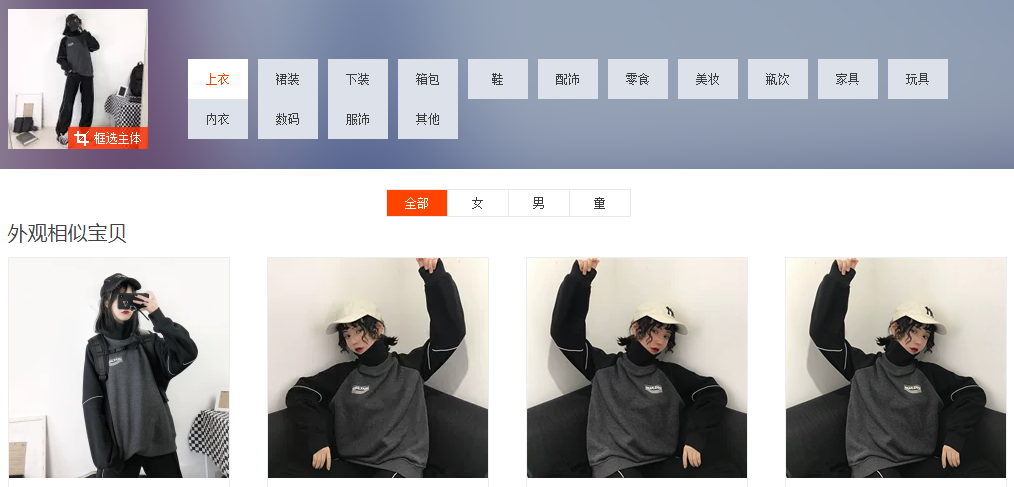
\includegraphics[width = 1\linewidth]{Img/tb.png}
  \caption{淘宝提供的以图搜图功能,用于检索同款商品}
  \label{fig:tb}
\end{figure*}

\section{国内外研究现状}

\subsection{基于视觉特征的服装检索}

服装检索的发展历史可以根据其核心方法分为两步,它们分别是基于文本和基于内容的服装检索方法。基于文
本的服装检索通过关键字或者更加自由形式的文本信息来描述商品,然后通过文本匹
配算法进行服装商品的检索,其本质是以文本搜图。目前,像服装购物平台淘宝等主流
电子商务网站检索服装图像都是以 TBIR(Text-based Image Retrieval)技术为主,TBIR
一般通过关键字检索,其特点是快速精准,但是随着服装种类与数量的不断迅速增长,
TBIR 的不足之处也开始显现出来:现在人们对于服装细节的要求越来越高,然而采用
关键字去标注服装图像无法全面准确的表示服装的细节信息;TBIR 需要人工的对海量
的服装图像做标注,对人力资源消耗较大;人工在标注时主观性比较大,难免有些偏差,这也会直接导致检索结果
的错误。因此,对基于内容的服装图像检索算法的研究很有必要性,CBIR 通过学习图
像的视觉语义特征进行检索,可以弥补 TBIR 的很多不足。

CBIR 算法首先会抽取图像的特征,然后将该特征和检索库里的特征对比,计算相
似度,并根据结果从大到小排序,从而可以得到最终的检索结果。初期的 CBIR 算法一般
致力于更好的提取服装的视觉特征,借助于服装本身在整个服装图像中的特异性,比如其款式多样、颜
色鲜明、细节突出等特点,相对与自然景象或者生活中其他常见物体等背景信息更加具
有区分度。从服装的这些特点中我们可以抽取服装的纹理、颜色、形状这三大视觉特征,
对这三种特征的提取是初期 CBIR 算法的主要方向:
\begin{itemize}
\item[1.]纹理特征:服装面料最为明显,最具区分性的特征就是纹理,纹理一般情况下以
图像的某种局部特性表现出来,纹理的多样性决定了服装的外在美观程度,更好的提取
服装图片的纹理特征十分有利于检索得到相似度高的服装图像。传统提取纹理特征的方
法主要有四种:频谱法、统计法、结构法和模型法。
纹理特征的提取算法最好具有旋转不变性, Ojala等人提出基于图像局部信息的LBP纹理分析方法,该方法虽然具有良好的旋转不变性,但没有很好
的利用图像的全局信息\cite{ojala2002multiresolution}
。Manthalkar等人的方法具有旋转不变性和尺度不变性,然而
该方法牺牲了纹理的方向信息\cite{manthalkar2003rotation}。

\item[2.] 颜色特征:颜色是服装的重要构成部分,是图像的一种显著的视觉特征,其对于
图像检索也一直是十分重要的特征。早期对颜色特征的提取主要通过统计图像像素点的
值,近阶段则是偏向于研究图像颜色信息空间分布的检索方法,Pass 等人统计图像中各
颜色最大连续区域的像素值,将其作为颜色特征\cite{pass1996comparing};Strieker 等人将图像划分,再分别
对划分后的各个子区域进行颜色特征的统计提取\cite{stricker1997spectral}。总体的来说,目前基于颜色信息
的检索方法主要考虑对全局以及局部颜色特征的抽取。

\item[3.] 形状特征:形状是服装款式如此丰富的重要原因,形状元素蕴含了服装的设计理念和
风格,其对于人的视觉感受也是十分重要的因素。形状特征的提取被广泛应用于 CBIR,
除了如何更好的提取形状特征之外,不同形状特征之间的相似度计算也是近来被探索的
课题。
对形状特征的提取注重关注服装图像的轮廓信息,以及更好的处理区域特征。轮廓
特征指服装的边界形状信息所包含的特征,相关参数有边界点、面积、周长等,相关研
究有 Livarinen 等人提出链码直方图\cite{iivarinen1997comparison};Berretti
等人提出基于平滑曲线分解特征等\cite{berretti2000retrieval}。区域特征指的是图像服装区域内部所包含的信
息,常用矩的方法, Chin等人提出几何不变矩,可以更好地提取形状特征\cite{teh1988image}。对形状特相似性度量的
研究:Peter 等提出 K 最近邻图\cite{kontschieder2009beyond};Bai 等人利用了形状特征之间的相似性与图之间
的相互关系,将形状特征间的相似性构建为图,更有效得去度量形状间相似性\cite{bai2010learning}。
\end{itemize}

\subsection{基于语义特征的服装检索}
传统的 CBIR 方法采用颜色、形状、纹理等较为底层的基于视觉的特征,使用的
分类器大多是浅层分类器,如支持向量机。这种基于底层视觉特征的检索系统和人类视
觉体系对图像的理解存在着语义鸿沟,即对于不同的图片,机器从低级的可视化特征得
到的相似性和人类视觉处理机制通过对语义特征的理解得到的相似性之间的鸿沟\cite{卢兴敬2008基于内容的服装图像检索技术研究及实现}。所以,即便图像检索
领域在对底层视觉特征的提取有了很大进展,提出了一系列不同的方法,但由于语义鸿
沟的存在,图像检索依然面临着巨大的挑战,我们希望机器可以像人一样理解识别图片
内容,则需要从更高层次去分析图片,现阶段最有希望解决这个语义鸿沟的技术是机器
学习。机器学习是一门涉及统计学、概率论、优化算法等领域的交叉学科,旨在研究如
何让计算机像人一样去学习新的知识,模仿人的行为,不断的通过学习提高自己。机器
学习算法的学习流程是:人为的将大量数据输入到计算机程序,让计算机去处理这些海
量数据,使其发现并总结出这些数据背后所蕴含的规律等隐含信息,机器学习的优势是
可以凭借计算机的高性能计算从大数据中学习得到人类无法轻易总结出的规律。21 世
纪以来,机器学习技术不断发展成熟,应用范围也从开始单纯的字符识别慢慢多样化,
比如生物信息中的基因大数据分析,金融行业中通过对历史数据规律的分析预测市场走
向。

在机器学习中,深度学习技术近年来得到了爆发性的发展,深度学习在计算机视觉、
自然语言处理、多媒体、语音识别等方向均带来了实质性的突破,显著的的推进了人工智能
领域的发展进程。深度学习作为机器学习领域的一个分支,起源于 80 年代的 BP \cite{rumelhart1988learning}神经网
络,这是一种对误差逆向传播的多层前馈神经网络,其核心思想是通过梯度下降法不断
优化网络,使得算法不断往误差的最小化方向参数调优。深度学习发展如此迅猛主要得
益于两个方面的原因:计算机的计算能力快速发展,神经网络的训练可以部署在 GPU
上并且可以并行训练,这使得大规模的神经网络可以训练;另一个原因则是大数据的快
速发展,训练数据是机器学习算法的核心之一,随着互联网的发展,日常产生的数据呈
指数级增长,这些海量的标注数据促进了深度学习模型的训练。相对于传统机器学习,
深度学习可以自动的找出分析问题所需要的重要特征,随着神经网络的加深,可以抽取
上层次的语义信息。深度网络中比较有代表性的是卷积神经网络,Lecun 等 提出的
LeNet-5\cite{lecun1998gradient} 在手写字符识别的任务上取得很大的成功,这使得卷积神经网络在学术界广受关注,2012
年 由Alex Krizhevsky 提出 的AlexNet\cite{krizhevsky2012imagenet}摘下了视觉领域竞赛 ILSVRC 2012 的桂冠,在
深度学习里颇具权威性的百万量级的 ImageNet\cite{deng2009imagenet} 数据集合上,且效果大幅度领先传统的方法,这成为卷积神经网
络的一个历史性时刻,AlexNet 之后,不断有新的卷积神经网络模型被提出,从 VGG\cite{simonyan2014very}、
GoogLeNet\cite{szegedy2015going}、Res-Net\cite{he2016deep} 到近期的 Res-NeXt\cite{xie2017aggregated}、SE-Net\cite{hu2018squeeze}。

和基于视觉特征类似,对于区域信息特征的学习是基于语义特征的服装检索一个重
要研究方向,CVPR2016 的工作 Fashion-Net\cite{liu2016deepfashion} 在服装检索中通过关键点信息来对局部特
征进行对齐操作,通过第一步预测出关节点,然后通过关键点信息和池化操作获得对应
的局部特征,这种做法可以较为准确的定位到服装所在区域,但是需要对于关键点的标
注数据进行训练,资源消耗较大。在服装检索的问题上,同款服装的不同图片的相似度
应大于不同款服装的相似度,因此度量学习在网络训练时被广泛使用。常用的度量学习
损失方法有对比损失(Contrastive loss)
、三元组损失(Triplet loss)
、困难样本采样三元
组损失(Triplet hard loss with batch hard mining, TriHard loss)等。除了以度量损失函数
作为网络训练的监督信息以外,服装的低层信息,比如颜色、纹理、形状等也常被作为
辅助监督,这种多任务学习的方式使得网络具有更强的表达能力,学习得到语义信息更
加丰富的特征。

\subsection{深度卷积网络}
目前情况下,包括图像检索在内的许多计算机视觉任务,在大部分情况下都会使用常用的基础分类网络作为其骨干网络充当特征提取器,这些主流的分类网络的性能已经在ImageNet得到证明。最经典的卷积神经网络是Yann LeCun在1998年设计并提出LeNet,这个用于识别手写字符的网络规模较小,但是包含了现在卷积神经网络的最基本组件:卷积层,池化层,全连接层。Alex Krizhevsky于2012年提出的AlexNet是卷积神经网络的一大步:AlexNet使用ReLU取代Sigmoid作为激活函数,成功解决了Sigmoid在网络较深时的梯度弥散问题;训练时采用了Dropout策略,随机忽略一部分神经元,可以有效避免模型的过拟合;引入了最大池化层而不是像之前只使用平均池化层,这有效的提升了特征的丰富性;使用CUDA加速神经网络训练,有效利用了GPU的计算能力。AlexNet被提出之后,深度学习飞速发展,越来越多性能优异的基础网络随之被提出,下面简要分析几个主流的基础网络:
\begin{itemize}
  \item [1.]VGG:相比AlexNet,VGG的一个改进是采用连续的几个3x3的卷积核代替AlexNet中的11x11或者5x5的较大卷积核。对于给定的感受野,采用堆积的小卷积核是优于采用大的卷积核,因为多层非线性层可以增加网络深度来保证学习更复杂的模式,此外小的卷积核也意味着更少的参数量,更低的计算复杂度。总结性的来说,VGG在控制计算量增长的同时将网络架构做的更深更宽,分类效果显著提升。\begin{figure}[h]
  \centering
  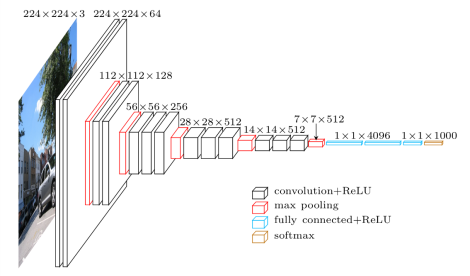
\includegraphics[width=10cm, height=6cm]{Img/vgg.png}
  \caption{VGG整体结构}
  \label{fig:vgg}
\end{figure}

\item [2.]Inception:又被称为GoogLeNet,实际上Inception指的是GoogLeNet的核心结构。一般来说提高网络表达能力最直接的方法就是增加网络的深度和宽度,但是直接这么做会带来一些问题:
\begin{itemize}
  \item [(1)]相对更深更宽的网络不可避免的会增加参数量,而过多的参数量容易导致过拟合。
  \item [(2)] 随着网络的深度的增加,由于深度学习本身学习机制的原因,误差在反向传播时会出现梯度消失或者称为梯度弥散的问题,导致网络很难优化。
  \item [(3)] 计算量增加,会消耗更多的计算资源。
\end{itemize}

Inception结构针对限制神经网络性能的主要问题对传统的卷积策略不断改进,Inception v1设计出了多路并行的卷积模块,不同分支的卷积核大小不同,分别有1x1,3x3,5x5三种尺度,这么做的好处是可以以不同大小的感受野去学习得到不同的特征,卷积操作之后,不同分支的特征通过拼接的方式做融合。
\begin{figure}[h]
  \centering
  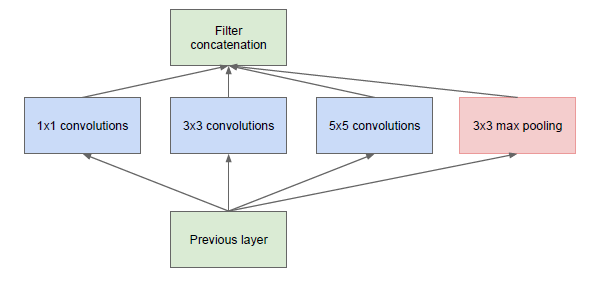
\includegraphics[width=13cm, height=6cm]{Img/inception-v1.png}
  \caption{Inception v1}
  \label{fig:inception-v1}
\end{figure}

Inception v2\cite{ioffe2015batch}基于Inception v1做了进一步的改进,提出了有重大意义的BN(Batch Normalization)。训练深度神经网络时,作者抛出一个叫做“Internal Covariate Shift”的问题,这个问题指在网络训练阶段,当前层的输入就是上一层的输出,在这个过程中,每训练一轮参数就会发生变化,对于一个网络相同的输入,前一层的输出却不一样,这就导致当前层的输入也不一样,BN的提出就是为了解决这个问题。在传统机器学习中,对图像提取特征之前,都会对图像做白化操作,即对输入数据变换成0均值、单位方差的正态分布,白化操作可以加快收敛,对于深度网络,每个隐层的输出都是下一个隐层的输入,即每个隐层的输入都可以做白化操作,BN就是在训练中的每个mini-batch上做了白化,可以有效防止梯度消失并加速网络训练。

\item [3.]ResNet:由微软研究院的Kaiming He等提出的ResNet,通过使用ResNet Unit成功训练出了152层的神经网络,其效果非常优异,在ILSVRC2015比赛中夺得头筹。

提出残差学习的思想。传统的卷积网络或者全连接网络在信息传递的时候或多或少会存在信息丢失,损耗等问题,同时还有导致梯度消失或者梯度爆炸,导致很深的网络无法训练。ResNet在一定程度上解决了这个问题,通过直接将输入信息绕道传到输出,保护信息的完整性,整个网络只需要学习输入、输出差别的那一部分,简化学习目标和难度。VGGNet和ResNet的对比如下图所示。ResNet最大的区别在于有很多的旁路将输入直接连接到后面的层,这种结构也被称为shortcut或者skip connections。

\begin{figure}[h]
  \centering
  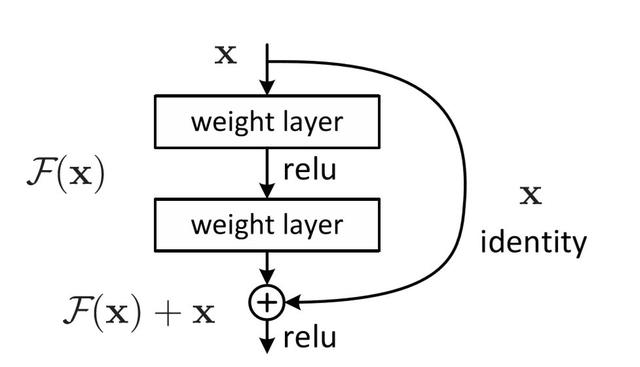
\includegraphics[width=10cm, height=6cm]{Img/resnet.jpg}
  \caption{ResNet 残差模块\cite{he2016deep}}
  \label{fig:resnet}
\end{figure}


\item [4.]SENet:近年来,为了提升网络性能,多数工作从空间纬度展开,比如Incepion使用
多尺度的卷积核以获取并聚合不同感受野的特征,另外比较具有代表性的有将注意力机制
引入到空间维度上去,这些工作都取得了很好的效果。而SENet则引入了另一种思路:是否可以考虑特征通道之间的关系以提升网络性能?SE是Squeeze-and-Excitation的缩写,
Squeeze和Excitation则是SENet核心模块的两个关键操作,模块具体流程如下:
\begin{itemize}
  \item [(1)] 对一个三维的特征图做Global average pooling,得到特征维度为${c\times1\times1}$,其中c为特征图的通道数,这个操作成为Squeeze。
  \item [(2)] 随后为两个FC层(Fully-connected-layer)去学习通道之间的相关性,其中第一个FC层将输入维度降低至原来的1/16,并经过ReLu,第二个FC层再将特征升至原来的维度。
  用两个FC层的好处是可以增加非线性以更好的建模通道相关性,并且可以大幅度减少参数量。
  \item [(3)] 最后通过Sigmoid将特征归一化至0到1之间,代表每个通道的重要程度,并将权重点乘至原特征图上。
\end{itemize}
\end{itemize}

\subsection{目标检测预处理}
服装检索这个任务在执行过程中常常需要用到目标检测,这是由任务的实际场景所决定的,训练深度模型的训练样本一般来自商家或者买家的拍摄图像,而拍摄得到的图像难免会包含
除了服装信息之外背景噪声,这个时候就需要目标检测在图像输入网络之前对其做预处理。目标检测是计算机视觉的基础任务之一,相较于分类任务,检测不仅需要识别图像中“有什么”,
还要判断所检测物体“在哪里”。以图\ref{fig:im-det}为例:这是来自买家拍摄的一张图,除了买家身上的裙子之外,图像中还有镜子、桌子、窗帘以及人体等不相关因素,
这种情形之下需要一个检测群装的检测器,检测的结果如图中的红色检测框所示,那么我们就可以去除绝大部分的噪声,得到只包含服装的图像。
\begin{figure}[h]
  \centering
  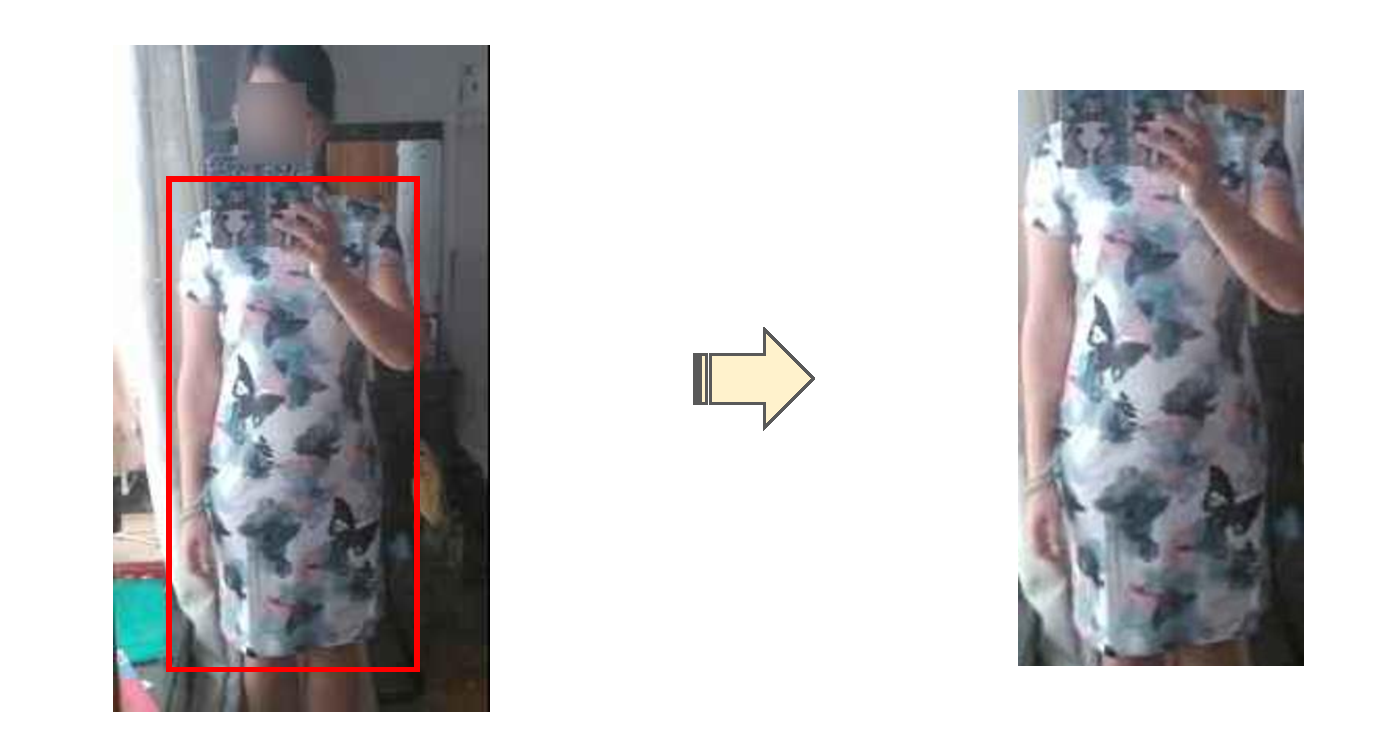
\includegraphics[width=0.8\linewidth]{Img/im-det.pdf}
  \caption{使用目标检测对检索图像预处理}
  \label{fig:im-det}
\end{figure}


在深度学习诞生之前,目标检测还是基于人工构建的特征,因此特征的表达能力十分有限,多数工作的重点集中在设计更好的检测算法上,从而弥补特征表达能力的不足。当时比较
有代表性的算法有:Viola-Jones检测器\cite{viola2001rapid,viola2004robust},在当时的计算条件下,首次实现了实时的人脸检测;
针对行人检测问题提出的HOG行人检测器\cite{dalal2005histograms};DPM算法及其改进\cite{felzenszwalb2008discriminatively,felzenszwalb2010cascade,felzenszwalb2010object}
将对整个物体的检测拆分为对多个部件的检测,最后再整合在一起,DPM算法里的很多思想一直延续至今,比如上下文信息以及困难样本等。

在深度学习诞生的前几年,目标检测的进度几乎停滞不前,首次将深度学习引入目标检测任务的工作是R-CNN\cite{girshick2014rich},这也标志着目标检测进入高速发展阶段。
R-CNN策略简单易懂,首先对输入图像提取了大量候选框(Object proposal),根据每个proposal对原图裁减,并缩放至统一之大小后输入AlexNet提取特征,最后对特征使用SVM分类。
R-CNN相较于DPM系列算法有着大幅度的提升,但是R-CNN算法的不足之处也较为明显:需要先提取特征,再用SVM分类,无法端到端的训练;不同的proposal可能会有大面积的重合区域,
重复提取特征造成了资源浪费而且导致检测速度较慢。

\begin{figure}[h]
  \centering
  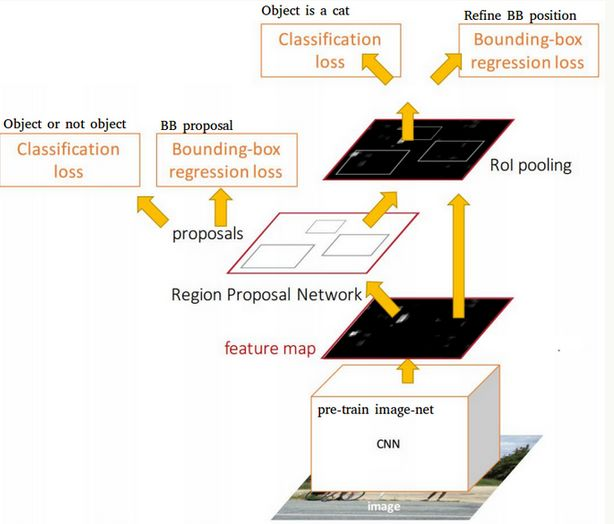
\includegraphics[width=0.7\linewidth]{Img/faster-rcnn.jpg}
  \caption{Faster R-CNN结构图\cite{ren2015faster}}
  \label{fig:faster-rcnn}
\end{figure}

在R-CNN的基础上,Girshick等人于2015年提出了Fast R-CNN\cite{girshick2015fast},实现了分类和回归的多任务学习,提升了性能的同时大幅度的加快了网络的训练速度以及检测速度
,Fast R-CNN的检测框生成方式依然是外部算法产生,所以并未实现端到端的训练。后来的Faster R-CNN\cite{ren2015faster}将候选框的提取也交给了网络去实现,
这也是Faster R-CNN的最大创新之处,即候选区域生成网络(RegionProposal Network),实现了真正的端到端的深度学习目标检测框架,对$640 \times 480$的输入图像可以做到17帧
每秒的检测速度。


\section{研究内容}
本课题采用 DeepFashion\cite{liu2016deepfashion} 数据集作为训练集,阿里巴巴 2017 大规模图像搜索大赛
的数据集作为测试集,共 300 万张测试图片。评价标准为上装,裙装和下装的检索 top4
命中率,对应的目标性能分别为 85\%、80\%、75\%。

对于服装图像检索这项任务,局部特征的学习与对齐一直是研究的重要方向,这也
是本课题面临的最大考验。此外,深度学习一直以来都有一个问题:训练好的模型在另
外一个域的性能会下降。基于这些问题,本课题的研究内容主要针对如下内容展开:(1)
探究度量学习以及多任务学习,以提升模型表达能力;(2)研究模型在不同域数据集
之间性能不一致的问题,提升模型泛化能力;(3)探索如何有效结合局部特征以及全局
特征,以及更加准确的局部区域对齐方式。据此,本文的主要贡献如下:
\begin{itemize}
  \item [1.] 引入注意力机制,让网络自适应的学习应该重点关注的局部区域。学习特征空间维度的权重分布,弱化图像中的噪音部分,且网络训练过程中除了类别标签外不需要额外的
    标注信息。采用多个分支并行的架构,可以使得每个分支关注的局部区域有所区别,进一步提升模型的表达能力。
    
    在此基础上,基于在线三元组损失提出跨域样本挖掘的方法。模型在实际使用场景下的输入数据与训练数据集常常有一定的区别,这种情况之下模型的性能往往达不到预期,因为来自不同域的数据集的数据
    分布与训练集本身就有差别。基于此,本文提出一种跨域挖掘样本的方式:先在原有的训练集训练出一个模型,然后在不同域的测试集中随机选择一定量的图像作为模型输入
    并在测试集做检索,每张输入图像都会得到Top K的排序输出,我们取这K张图片中排序相对靠前的图像作为和输入图像的同款服装样本,排序靠后的作为非同款样本,最后把这些样本
    放入原有的训练集训练。通过这种方式,模型可以更好的适应测试集的数据分布,进而有效提升在测试集的表现。
  
  \item [2.] 提出基于特征图的多粒度切分方法,大幅度增强特征的局部表达能力。分类任务一般基于整幅图的全局特征去做,本文在保留全局特征分类做法的基础上,增加了局部特征分类的分支,
    采用切分的方式,对特征图切分为N等份,每一块局部特征经过Global Pooling之后用类别标签去做监督。另外,使用不同大小的N作切分,多粒度的切分分支并行训练,进一步提升模型的性能。

    提出环形切分的策略,首先通过环形的切分方式,得到环形的特征块,对每快特征做环形的池化,可以有效解决实际场景常见的旋转问题,结合横向切分和纵向切分,
    使得网络对局部特征的学习更加全面。

\end{itemize}

\section{论文组织结构}
本文共分为四章,各章节内容安排如下:

第一章为绪论,介绍了本工作的研究背景和意义,简要叙述了有关服装检索任务的国内外研究现状,列出了本文的研究内容以及贡献,并对论文整体的结构安排做了梳理。

第二章介绍基于注意力机制的局部对齐网络,通过空间注意力和通道注意力的结合抓取局部信息,网络设计为多个局部分支并行的结构,用于提取不同的局部特征。
另外介绍了一种基于本网络的跨域样本挖掘算法,可以增强模型跨域的泛化能力。实验部分介绍了实验数据集以及评价指标,并可视化了不同局部分支的注意力分布。

第三章介绍基于多粒度切分的局部对齐网络,分析了对特征图切分的动机,提出环形切分和多粒度切分的策略,有效提升模型对关键局部特征的抓取能力,丰富了特征的语义表达能力。

第四章为结束语,对论文所做的工作进行全面的总结,并对未来的工作方向作出分析和展望。

\chapter{相关工作}



\section{基于视觉特征的服装检索}

服装检索的发展经历了两个阶段,分别是基于文本和基于内容的服装检索。基于文
本的服装检索通过关键字或者更加自由形式的文本信息来描述商品,然后通过文本匹
配算法进行服装商品的检索,其本质是以文本搜图。目前,像服装购物平台淘宝等主流
电子商务网站检索服装图像都是以 TBIR(Text-based Image Retrieval)技术为主,TBIR
一般通过关键字检索,其特点是快速精准,但是随着服装种类与数量的不断迅速增长,
TBIR 的不足之处也开始显现出来:现在人们对于服装细节的要求越来越高,然而采用
关键字去标注服装图像无法全面准确的表示服装的细节信息;TBIR 需要人工的对海量
的服装图像做标注,工作量很大;人工标注有时会缺乏客观性,这会直接导致检索结果
的偏差。因此,对基于内容的服装图像检索算法的研究很有必要性,CBIR 通过学习图
像的视觉语义特征进行检索,可以弥补 TBIR 的很多不足。

CBIR 算法首先会抽取图像的特征,然后将该特征和检索库里的特征对比,计算相
似度,按照相似性的大小来排序从而可以得到最终的检索结果。初期的 CBIR 算法一般
致力于更好的提取服装的视觉特征,服装是整个服装图像中的主体,因其款式多样、颜
色鲜明、细节突出等特点,相对与自然景象或者生活中其他常见物体等背景信息更加具
有区分度。从服装的这些特点中我们可以抽取服装的纹理、颜色、形状这三大视觉特征,
对这三种特征的提取是初期 CBIR 算法的主要方向:
\begin{itemize}
\item[1.]纹理特征:服装面料最为明显,最具区分性的特征就是纹理,纹理一般情况下以
图像的某种局部特性表现出来,纹理的多样性决定了服装的外在美观程度,更好的提取
服装图片的纹理特征十分有利于检索得到相似度高的服装图像。传统提取纹理特征的方
法主要有四种:频谱法、统计法、结构法和模型法。
纹理特征的提取算法最好具有旋转不变性,Ojala等人提出的LBP纹理分析方法具有旋转不变性的优点,但该方法只使用了服装图像的局部信息去提取特征,没有很好
的利用图像的全局信息\cite{ojala2002multiresolution}
。Manthalkar等人的方法具有旋转不变性和尺度不变性,然而
该方法牺牲了纹理的方向信息\cite{manthalkar2003rotation}。

\item[2.] 颜色特征:颜色是服装的重要构成部分,是图像的一种显著的视觉特征,其对于
图像检索也一直是十分重要的特征。早期对颜色特征的提取主要通过统计图像像素点的
值,近阶段则是偏向于研究图像颜色信息空间分布的检索方法,Pass 等人统计图像中各
颜色最大连续区域的像素值,将其作为颜色特征\cite{pass1996comparing};Strieker 等人将图像划分,再分别
对划分后的各个子区域进行颜色特征的统计提取\cite{stricker1997spectral}。总体的来说,目前基于颜色信息
的检索方法主要考虑对全局以及局部颜色特征的抽取。

\item[3.] 形状特征:形状是决定服装款式多样性的重要因素,蕴含了服装的设计理念和
风格,其对于人的视觉感受也是十分重要的因素。形状特征的提取被广泛应用于 CBIR,
除了如何更好的提取形状特征之外,不同形状特征之间的相似度计算也是近来被探索的
课题。
对形状特征的提取注重关注服装图像的轮廓信息,以及更好的处理区域特征。轮廓
特征指服装的边界形状信息所包含的特征,相关参数有边界点、面积、周长等,相关研
究有 Livarinen 等人提出链码直方图\cite{iivarinen1997comparison};Berretti
等人提出基于平滑曲线分解特征等\cite{berretti2000retrieval}。区域特征指的是图像服装区域内部所包含的信
息,常用矩的方法, Chin等人提出几何不变矩,可以更好地提取形状特征\cite{teh1988image}。对形状特相似性度量的
研究:Peter 等提出 K 最近邻图\cite{kontschieder2009beyond};Bai 等人利用了形状特征之间的相似性与图之间
的相互关系,将形状特征间的相似性构建为图,更有效得去度量形状间相似性\cite{bai2010learning}。
\end{itemize}

\section{基于语义特征的服装检索}
传统的 CBIR 方法采用颜色、形状、纹理等视觉特征,这些特征较为底层,使用的
分类器大多是浅层分类器,如支持向量机。这种基于底层视觉特征的检索系统和人类视
觉体系对图像的理解存在着语义鸿沟,即对于不同的图片,机器从低级的可视化特征得
到的相似性和人从高级的语义特征得到的相似性之间的不同\cite{卢兴敬2008基于内容的服装图像检索技术研究及实现}。所以,即便图像检索
领域在对底层视觉特征的提取有了很大进展,提出了一系列不同的方法,但由于语义鸿
沟的存在,图像检索依然面临着巨大的挑战,我们希望机器可以像人一样理解识别图片
内容,则需要从更高层次去分析图片,现阶段最有希望解决这个语义鸿沟的技术是机器
学习。机器学习是一门涉及统计学、概率论、优化算法等领域的交叉学科,旨在研究如
何让计算机像人一样去学习新的知识,模仿人的行为,不断的通过学习提高自己。机器
学习算法的学习流程是:人为的将大量数据输入到计算机程序,让计算机去处理这些海
量数据,使其发现并总结出这些数据背后所蕴含的规律等隐含信息,机器学习的优势是
可以凭借计算机的高性能计算从大数据中学习得到人类无法轻易总结出的规律。21 世
纪以来,机器学习技术不断发展成熟,应用范围也从开始单纯的字符识别慢慢多样化,
比如生物信息中的基因大数据分析,金融行业中通过对历史数据规律的分析预测市场走
向。

在机器学习中,深度学习技术近年来得到了爆发性的发展,深度学习在计算机视觉、
自然语言处理、多媒体、语音识别等方向均取得了巨大的成功,极大的推动了人工智能
领域的发展进程。深度学习作为机器学习领域的一个分支,起源于 80 年代的 BP \cite{rumelhart1988learning}神经网
络,这是一种对误差逆向传播的多层前馈神经网络,其核心思想是通过梯度下降法不断
优化网络,使得算法不断往误差的最小化方向参数调优。深度学习发展如此迅猛主要得
益于两个方面的原因:计算机的计算能力快速发展,神经网络的训练可以部署在 GPU
上并且可以并行训练,这使得大规模的神经网络可以训练;另一个原因则是大数据的快
速发展,训练数据是机器学习算法的核心之一,随着互联网的发展,日常产生的数据呈
指数级增长,这些海量的标注数据促进了深度学习模型的训练。相对于传统机器学习,
深度学习可以自动的找出分析问题所需要的重要特征,随着神经网络的加深,可以抽取
上层次的语义信息。深度网络中比较有代表性的是卷积神经网络,Lecun 等 提出的
LeNet-5\cite{lecun1998gradient} 在手写字符识别领域的成功应用引起了学术界对于卷积神经网络的关注,2012
年 Alex Krizhevsky 提出 AlexNet\cite{krizhevsky2012imagenet},一举摘下了视觉领域竞赛 ILSVRC 2012 的桂冠,在
百万量级的 ImageNet\cite{deng2009imagenet} 数据集合上,效果大幅度超过传统的方法 [7],这成为卷积神经网
络的一个历史性时刻,AlexNet 之后,不断有新的卷积神经网络模型被提出,从 VGG\cite{simonyan2014very}、
GoogLeNet\cite{szegedy2015going}、Res-Net\cite{he2016deep} 到近期的 Res-NeXt\cite{xie2017aggregated}、SE-Net\cite{hu2018squeeze}。

和基于视觉特征类似,对于区域信息特征的学习是基于语义特征的服装检索一个重
要研究方向,CVPR2016 的工作 Fashion-Net\cite{liu2016deepfashion} 在服装检索中通过关键点信息来对局部特
征进行对齐操作,通过第一步预测出关节点,然后通过关键点信息和池化操作获得对应
的局部特征,这种做法可以较为准确的定位到服装所在区域,但是需要对于关键点的标
注数据进行训练,资源消耗较大。在服装检索的问题上,同款服装的不同图片的相似度
应大于不同款服装的相似度,因此度量学习在网络训练时被广泛使用。常用的度量学习
损失方法有对比损失(Contrastive loss)
、三元组损失(Triplet loss)
、困难样本采样三元
组损失(Triplet hard loss with batch hard mining, TriHard loss)等。除了以度量损失函数
作为网络训练的监督信息以外,服装的低层信息,比如颜色、纹理、形状等也常被作为
辅助监督,这种多任务学习的方式使得网络具有更强的表达能力,学习得到语义信息更
加丰富的特征。

\section{深度卷积网络}
目前情况下,包括图像检索在内的许多计算机视觉任务,在大部分情况下都会使用常用的基础分类网络作为其骨干网络充当特征提取器,这些主流的分类网络的性能已经在ImageNet得到证明。最经典的卷积神经网络是Yann LeCun在1998年设计并提出LeNet,这个用于识别手写字符的网络规模较小,但是包含了现在卷积神经网络的最基本组件:卷积层,池化层,全连接层。Alex Krizhevsky于2012年提出的AlexNet是卷积神经网络的一大步:AlexNet使用ReLU取代Sigmoid作为激活函数,成功解决了Sigmoid在网络较深时的梯度弥散问题;训练时采用了Dropout策略,随机忽略一部分神经元,可以有效避免模型的过拟合;引入了最大池化层而不是像之前只使用平均池化层,这有效的提升了特征的丰富性;使用CUDA加速神经网络训练,有效利用了GPU的计算能力。AlexNet被提出之后,深度学习飞速发展,越来越多性能优异的基础网络随之被提出,下面简要分析几个主流的基础网络:
\begin{itemize}
  \item [1.]VGG:相比AlexNet,VGG的一个改进是采用连续的几个3x3的卷积核代替AlexNet中的11x11或者5x5的较大卷积核。对于给定的感受野,采用堆积的小卷积核是优于采用大的卷积核,因为多层非线性层可以增加网络深度来保证学习更复杂的模式,此外小的卷积核也意味着更少的参数量,更低的计算复杂度。总结性的来说,VGG在控制计算量增长的同时将网络架构做的更深更宽,分类效果显著提升。\begin{figure}[h]
  \centering
  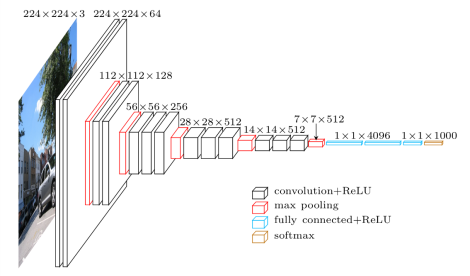
\includegraphics[width=10cm, height=6cm]{Img/vgg.png}
  \caption{VGG整体结构}
  \label{fig:vgg}
\end{figure}

\item [2.]Inception:又被称为GoogLeNet,实际上Inception指的是GoogLeNet的核心结构。一般来说提高网络表达能力最直接的方法就是增加网络的深度和宽度,但是直接这么做会带来一些问题:
\begin{itemize}
  \item [(1)]相对更深更宽的网络不可避免的会增加参数量,而过多的参数量容易导致过拟合。
  \item [(2)] 随着网络的深度的增加,反向传播时会出现梯度消失的问题,导致网络很难优化。
  \item [(3)] 计算量增加,会消耗更多的计算资源。
\end{itemize}

Inception结构针对限制神经网络性能的主要问题对传统的卷积策略不断改进,Inception v1设计出了多路并行的卷积模块,不同分支的卷积核大小不同,分别有1x1,3x3,5x5三种尺度,这么做的好处是可以以不同大小的感受野去学习得到不同的特征,卷积操作之后,不同分支的特征通过拼接的方式做融合。
\begin{figure}[h]
  \centering
  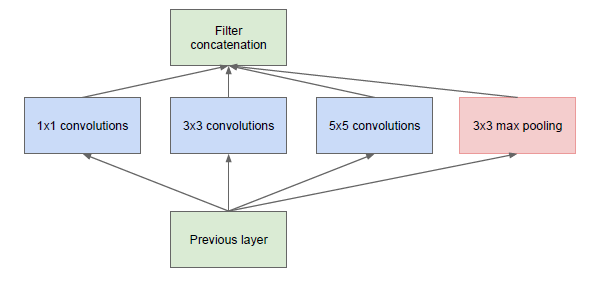
\includegraphics[width=13cm, height=6cm]{Img/inception-v1.png}
  \caption{Inception v1}
  \label{fig:inception-v1}
\end{figure}

Inception v2\cite{ioffe2015batch}基于Inception v1做了进一步的改进,提出了有重大意义的BN(Batch Normalization)。训练深度神经网络时,作者抛出一个叫做“Internal Covariate Shift”的问题,这个问题指在训练过程中,第n层的输入就是第n-1层的输出,在训练过程中,每训练一轮参数就会发生变化,对于一个网络相同的输入,但n-1层的输出却不一样,这就导致第n层的输入也不一样,BN的提出就是为了解决这个问题。在传统机器学习中,对图像提取特征之前,都会对图像做白化操作,即对输入数据变换成0均值、单位方差的正态分布,卷积神经网络的输入就是图像,白化操作可以加快收敛,对于深度网络,每个隐层的输出都是下一个隐层的输入,即每个隐层的输入都可以做白化操作,BN就是在训练中的每个mini-batch上做了白化,可以有效防止梯度消失并加速网络训练。

\item [3.]ResNet:由微软研究院的Kaiming He等提出的ResNet,通过使用ResNet Unit成功训练出了152层的神经网络,其效果非常优异,在ILSVRC2015比赛中夺得头筹。

提出残差学习的思想。传统的卷积网络或者全连接网络在信息传递的时候或多或少会存在信息丢失,损耗等问题,同时还有导致梯度消失或者梯度爆炸,导致很深的网络无法训练。ResNet在一定程度上解决了这个问题,通过直接将输入信息绕道传到输出,保护信息的完整性,整个网络只需要学习输入、输出差别的那一部分,简化学习目标和难度。VGGNet和ResNet的对比如下图所示。ResNet最大的区别在于有很多的旁路将输入直接连接到后面的层,这种结构也被称为shortcut或者skip connections。

\begin{figure}[h]
  \centering
  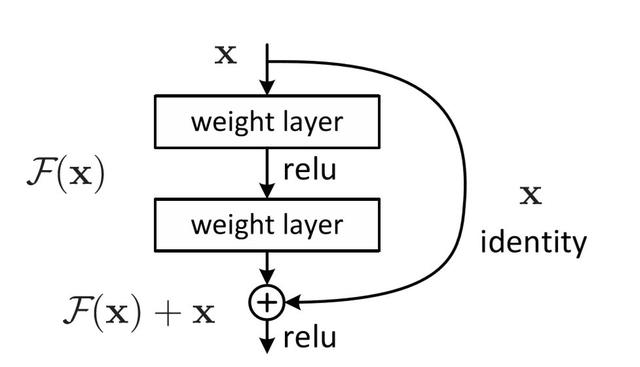
\includegraphics[width=10cm, height=6cm]{Img/resnet.jpg}
  \caption{ResNet 残差模块\cite{he2016deep}}
  \label{fig:resnet}
\end{figure}


\item [4.]SENet:近年来,为了提升网络性能,多数工作从空间纬度展开,比如Incepion使用
多尺度的卷积核以获取并聚合不同感受野的特征,另外比较具有代表性的有将注意力机制
引入到空间维度上去,这些工作都取得了很好的效果。而SENet则引入了另一种思路:是否可以考虑特征通道之间的关系以提升网络性能?SE是Squeeze-and-Excitation的缩写,
Squeeze和Excitation则是SENet核心模块的两个关键操作,模块具体流程如下:
\begin{itemize}
  \item [(1)] 对一个三维的特征图做Global average pooling,得到特征维度为${c\times1\times1}$,其中c为特征图的通道数,这个操作成为Squeeze。
  \item [(2)] 随后为两个FC层(Fully-connected-layer)去学习通道之间的相关性,其中第一个FC层将输入维度降低至原来的1/16,并经过ReLu,第二个FC层再将特征升至原来的维度。
  用两个FC层的好处是可以增加非线性以更好的建模通道相关性,并且可以大幅度减少参数量。
  \item [(3)] 最后通过Sigmoid将特征归一化至0到1之间,代表每个通道的重要程度,并将权重点乘至原特征图上。
\end{itemize}
\end{itemize}

\section{目标检测}
服装检索这个任务在执行过程中常常需要用到目标检测,这是由任务的实际场景所决定的,训练深度模型的训练样本一般来自商家或者买家的拍摄图像,而拍摄得到的图像难免会包含
除了服装信息之外背景噪声,这个时候就需要目标检测在图像输入网络之前对其做预处理。目标检测是计算机视觉的基础任务之一,相较于分类任务,检测不仅需要识别图像中“有什么”,
还要判断所检测物体“在哪里”。以图\ref{fig:im-det}为例:这是来自买家拍摄的一张图,除了买家身上的裙子之外,图像中还有镜子、桌子、窗帘以及人体等不相关因素,
这种情形之下需要一个检测群装的检测器,检测的结果如图中的红色检测框所示,那么我们就可以去除绝大部分的噪声,得到只包含服装的图像。
\begin{figure}[h]
  \centering
  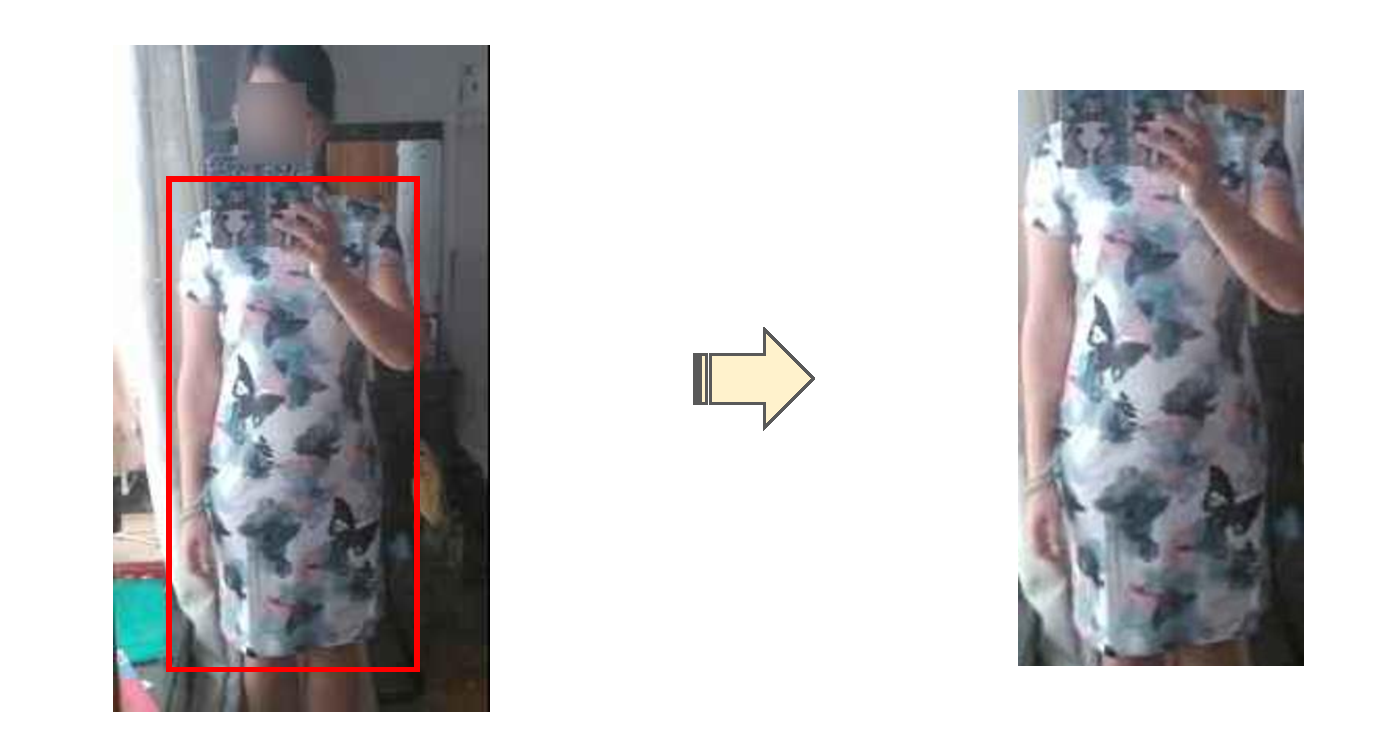
\includegraphics[width=0.8\linewidth]{Img/im-det.pdf}
  \caption{使用目标检测对检索图像预处理}
  \label{fig:im-det}
\end{figure}


在深度学习诞生之前,目标检测还是基于人工构建的特征,因此特征的表达能力十分有限,多数工作的重点集中在设计更好的检测算法上,从而弥补特征表达能力的不足。当时比较
有代表性的算法有:Viola-Jones检测器\cite{viola2001rapid,viola2004robust},在当时的计算条件下,首次实现了实时的人脸检测;
针对行人检测问题提出的HOG行人检测器\cite{dalal2005histograms};DPM算法及其改进\cite{felzenszwalb2008discriminatively,felzenszwalb2010cascade,felzenszwalb2010object}
将对整个物体的检测拆分为对多个部件的检测,最后再整合在一起,DPM算法里的很多思想一直延续至今,比如上下文信息以及困难样本等。

在深度学习诞生的前几年,目标检测的进度几乎停滞不前,首次将深度学习引入目标检测任务的工作是R-CNN\cite{girshick2014rich},这也标志着目标检测进入高速发展阶段。
R-CNN策略简单易懂,首先对输入图像提取了大量候选框(Object proposal),根据每个proposal对原图裁减,并缩放至统一之大小后输入AlexNet提取特征,最后对特征使用SVM分类。
R-CNN相较于DPM系列算法有着大幅度的提升,但是R-CNN算法的不足之处也较为明显:需要先提取特征,再用SVM分类,无法端到端的训练;不同的proposal可能会有大面积的重合区域,
重复提取特征造成了资源浪费而且导致检测速度较慢。

\begin{figure}[h]
  \centering
  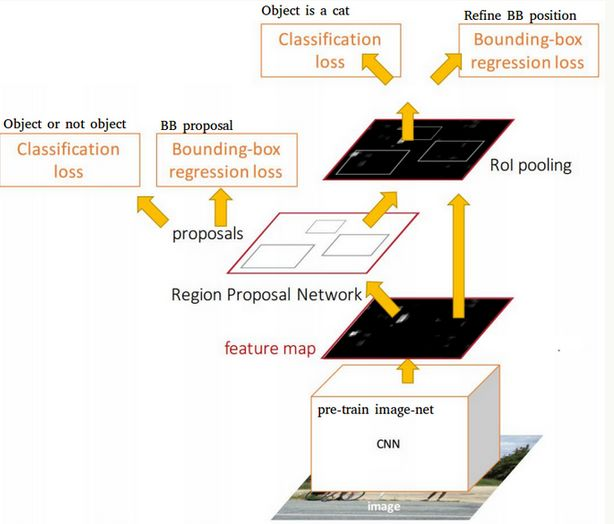
\includegraphics[width=0.7\linewidth]{Img/faster-rcnn.jpg}
  \caption{Faster R-CNN结构图\cite{ren2015faster}}
  \label{fig:faster-rcnn}
\end{figure}

在R-CNN的基础上,Girshick等人于2015年提出了Fast R-CNN\cite{girshick2015fast},实现了分类和回归的多任务学习,提升了性能的同时大幅度的加快了网络的训练速度以及检测速度
,Fast R-CNN的检测框生成方式依然是外部算法产生,所以并未实现端到端的训练。后来的Faster R-CNN\cite{ren2015faster}将候选框的提取也交给了网络去实现,
这也是Faster R-CNN的最大创新之处,即候选区域生成网络(RegionProposal Network),实现了真正的端到端的深度学习目标检测框架,对$640 \times 480$的输入图像可以做到17帧
每秒的检测速度。



\chapter{基于注意力机制的局部对齐网络}

\section{引言}
基于深度学习的服装检索网络一般可以概括为两个子网络:表示和匹配。表示网络即特征提取器,一般使用在ImageNet预训练的主流深度卷积网络,比如VGG、ResNet等主流骨干网络;
匹配网络对所提取特征进一步学习,以获得更适合服装检索这个任务的特征。特征提取器输出的特征经过Pooling之后得到一个向量之后,一般都会引入度量学习去做监督,
使同款的服装特征相似度提高,不同款的服装特征相似度降低,特征的相似度或者距离衡量常用余弦相似度。
常用的度量学习损失有Contrastive loss\cite{hadsell2006dimensionality}、Triplet loss\cite{schroff2015facenet}等,其公式分别如下所示

\textbf{contrastive 公式}

\textbf{triplet 公式}

大家在早期对服装检索的研究主要关注在全局信息上,即对整幅图提取一个全局的特征,但是后来这种方式遇到了瓶颈,大家开始慢慢把研究的方向转向对局部特征的学习与表示。
对于服装图像来说,全局信息包含了更加丰富的语义信息,但是对局部信息的抽取也非常有帮助,因为不同款式的服装有的时候仅仅有着细微的差别,在全局特征中,这些重要
但是不明显或者所占区域比例较小的局部信息会被Average Pooling稀释掉,如果可以通过某种方式将这个区域的特征单独提取出来,或者强化这个局部区域的特征强度,
对检索结果将会带来巨大的收益。比较常用的局部特征提取方法有对输入图像的切分\cite{varior2016siamese},或者网格\cite{li2014deepreid}等,这种方式直接获取局部特征
比较简单直接,但是也有其相应的不足之处:同款服装的不同拍摄图像摆放位置及形状不一定相同,两幅图的局部特征并不能很好的对齐。
Fashion-Net使用关键点信息协助局部的定位,网络第一阶段先生成对关键点位置的预测,第二阶段根据关键点位置对局部信息Pooling。通过关键点的方式可以很好的解决局部部件对齐
的问题,但是这个方法需要训练样本有对应关键点的标注信息,带来的资源消耗较大。

近年来,注意力机制(Attention Mechanism)在深度学习的各个领域都被广泛的使用,从自然语言处理到语音识别再到计算机视觉,都很容易看到注意力模型的存在。深度学习中的
注意力机制其实借鉴自人类视觉系统的注意力机制。人类的视觉注意力机制的本质是我们大脑的一种信号处理机制,首先对眼睛观测到的图像做全局的扫描和理解,分析之后会把注意力
放在需要重点关注的区域,从而抓取更多的细节信息,一定程度上屏蔽相对无关的信息,人的视觉注意力机制有效的提高了对视觉信息的理解效率和效果。在计算机视觉领域,
注意力模块往往指一个额外的网络模块,这个模块可以给输入的信息分配不同的权重之后再输出,特殊条件下,如果权重大小只能是0或者1时,就包括了切分或者网格的处理方式,
本节中的注意力机制特指软注意力机制(Soft Attention),即注意力权重为0到1之间的任意值。注意力模块可以直接嵌入到神经网络之中的,Soft Attention的权重输出是可微的,
所以整个模型可以进行端到端的训练。

\section{方法与实现}
\subsection{度量学习}
服装检索任务的目标是在由很多款式服装图像组成的检索库中找到和检索图片(query)相同款式的服装。这个任务可以被看作一种排序问题:给定一个query,那么检索库中和query
相同款式的服装相对于与其不同款式的服装应当和query更加相似。

基于此,本方法引入度量学习训练模型,训练样本组成方式如下:对于一个批次(Batch)的样本${\mathcal{B} = \{I_{1},I_{2},\cdots,I_{N}\}}$,我们从中组成一系列三元组,
${\mathcal{T} = \{(I_{a},I_{p},I_{n})\}}$,其中($I_{a},I_{p}$)是一对正样本对,表示这是来自同一款服装的两幅照片;($I_{a},I_{n}$)是一对负样本对,表示来自不同款式服装的
两幅照片。

由于检索任务的本质是一个排序问题,我们使用三元组损失(Triplet loss)函数优化网络,其数学表达式为:
\begin{equation}
\label{eq:partnet:1}
\mathcal{L}(I_{a},I_{p},I_{n}) = \max \{d(h(I_{a}),h(I_{p})) - d(h(I_{a}),h(I_{n})) + m,0\}
\end{equation}
这里$(I_{a},I_{p},I_{n}) \in \mathcal{T}$,$m$(margin)是我们认为负样本对之间的距离和正样本对之间应该有的距离差值,借鉴已有的工作\cite{schroff2015facenet},
在我们的实现中,$m$取了0.2。$d(\mathbf{x},\mathbf{y})=\left\|{\mathbf{x} - \mathbf{y}}\right\|_{2}$,代表了欧几里得距离,即欧式距离。$h(I)$代表将图像$I$输入网络并提取得到其特征。
所以我们可以得到如下完整的损失函数定义:
\begin{equation}
\label{eq:partnet:2}
\mathcal{L}(\mathcal{T}) = \frac{1}{\left|\mathcal{T}\right|} \sum_{(I_{a},I_{p},I_{n}) \in \mathcal{T}} \mathcal{L}(I_{a},I_{p},I_{n})
\end{equation}
公式里的$\left|\mathcal{T}\right|$代表这个Batch里所包含所有三元组的个数。

\subsection{局部对齐网络}
网络的第一阶段是一个特征提取器,这个特征提取器是一个深度全卷积神经网络(FCN),其输出是一个特征图,随后将其作为局部特征提取网络的输入,由其提取并输出局部特征。
与直接对输入图像做空间上的水平、竖直切分或者使用网格切分的方式不同,我们的目的是提取对齐之后的局部特征。

局部对齐网络如图\ref{fig:partnet}所示,包含了几个分支,每个分支都以FCN的输出作为输入,并检测到一个具有判别力的独立的局部区域,最后将这个区域的特征提取并输出。
我们将FCN所提取的特征图用一个三维的张量\textbf{T}表示,其每个维度大小为$w\times h \times c$,代表宽度为$w$,长度为$h$,通道数为$c$的张量。局部对齐网络的每个分支
都会生成一个二维的掩膜$M_{i}$,$i$代表第$i$个分支,其大小为$w\times h$,$M(x,y)$的大小表示$(x,y)$这个区域的特征对应的权重。
那么对于第$i$个分支来说,其输出特征$\textbf{T}_{i}$可表示为如下形式:
\begin{equation}
\label{eq:partnet:3}
\textbf{T}_{i}(x,y,c)=\textbf{T}(x,y,c) \times M_{i}(x,y)
\end{equation}
得到$\textbf{T}_{i}$之后,会通过全局平均池化(Global average pooling)操作得到一个向量,$\textbf{f}_{i}=AveragePooling(\textbf{T}_{i})$。
随后用一个线性降维层对这个向量降维,降维层采用全连接层实现,$\bar{\textbf{f}_{i}}=\textbf{W}_{FC_{i}}\textbf{f}_{i}$。接下来,我们将来自所有分支的局部特征拼接起来:
\begin{equation}
\label{eq:partnet:4}
\textbf{f}=[\bar{\textbf{f}_{1}}^\top,\bar{\textbf{f}_{2}}^\top,\cdots,\bar{\textbf{f}_{N}}^\top]^\top
\end{equation}
最后对拼接后的特征做$L_{2}$归一化,得到公式\ref{eq:partnet:1}中的$h(I)$。
\begin{figure}[h]
  \centering
  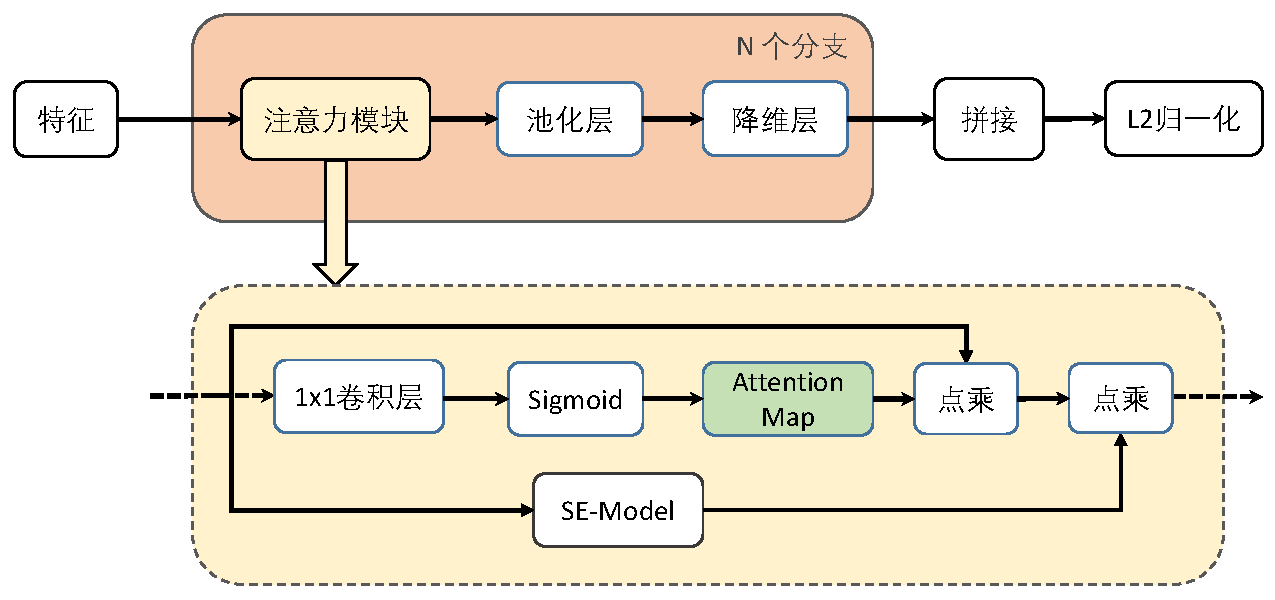
\includegraphics[width=1.0\linewidth]{Img/part.pdf}
  \caption{局部对齐网络的整体架构}
  \label{fig:partnet}
\end{figure}

\subsection{注意力模块}
本小节介绍如图\ref{fig:partnet}中所示的注意力模块。在局部对齐网络中,每一个分支都会生成一个掩膜$M_{i}$,这个掩膜的生成也是局部对齐的关键,其生成过程基于注意力机制,
我们称之为注意力模块。提出的注意力模块包括两个子模块:空间注意力模块和通道注意力模块。空间注意力模块学习空间维度的注意力分布;通道注意力模块则借鉴SENet的思想,
认为通道间具有互相依赖的关系,学习通道维度上的权重分布可以有效挖掘这种依赖关系以提升网络表达能力。




\bibliographystyle{Biblio/seuthesix} 
\bibliography{Biblio/ref}       
\end{document}
